\chapter{Experimentación y evaluación}
%-----------------------------------------------
% 5.1 Scientific workflows
%-----------------------------------------------
\todo[inline]{necesitas una introducción al capítulo, lo que vas a contar. Es lo mismo que pone en Trees Maps and theorems. Además, deberías empezar diciendo: esto es lo que hace un científico cuando construye y ejecuta un workflow de datos. No se entiende mucho esta sección.}

\section{Experimentos computacionales}\label{s5.1}

Para validar la propuesta y su aplicación en el contexto de workflows científicos, se ha seleccionado un subconjunto de workflows y WMSs\todo[inline]{dónde está definido esto de WMS?}. 
El subconjunto ha sido seleccionado bajo los criterios de: nivel de utilización de WMS, la diversidad de lenguajes utilizados en el conjunto, y disponibilidad de los materiales del workflow. 

Los materiales de workflow son: los datos, el código y la documentación. La documentación permite el estudio de los componentes de software necesarios para la ejecución del ambiente. Y los datos y el código permiten la ejecución obtención de los resultados.
Además para entender los requisitos del workflow, se inspecciona la las anotaciones manuales generadas por WICUS \cite{santana2017reproducibility} para el workflow seleccionado.
Luego, Para cada WMS, se construye una imagen estándar. En consecuencia, un investigador puede importar esta imagen e instalar los componentes de software relacionados con el workflow.
Esto se puede conseguir utilizando la instrucción \texttt{FROM} de Dockerfile. Por ejemplo, el workflow SoyKB utiliza Pegasus como WMS. Por lo tanto, la imagen SoyKb importa la imagen Pegasus lo cual permite no almacenar copia de las capas de Pegasus por cada workflow.
En caso que el WMSs no distribuya su software utilizando Docker, se construye las imágenes, los archivos necesarios como configuraciones y el DeploymentPlan (Dockerfile).\todo[inline]{cómo? no se supone que nosotros generamos esas anotaciones usando nuestra ontología que extiende la de wicus?}.  Para cada flujo de trabajo los archivos están disponibles en nuestros repositorios. \footnote{https://github.com/dockerpedia}.
Además, cada DeploymentFile incluye información sobre la imagen utilizando el estándar de la Open Container Initiative \footnote{\url{https://www.opencontainers.org/}} Esta información es:

\begin{description}
   \item[org.opencontainers.image.created:] fecha y hora en la que se construyó la imagen (string, fecha y hora según la definición de RFC 3339).
    \item [org.opencontainers.image.authors] datos de contacto de las personas u organizaciones responsables de la imagen (lista de forma libre)).
    \item [org.opencontainers.image.url] URL para encontrar más información sobre la imagen (string).
    \item [org.opencontainers.image.documentation] URL para obtener documentación sobre la imagen (string).
    \item [org.opencontainers.image.source] URL para obtener el código fuente para construir la imagen (string).
    \item [org.opencontainers.image.version] versión del software empaquetado
        La versión puede coincidir con una etiqueta o tag en el repositorio de código fuente versión podría ser compatible con el versionado semántico.
    \item [org.opencontainers.image.revision] Identificador de revisión de control de origen para el software empaquetado.
    \item [org.opencontainers.image.vendor] Nombre de la entidad distribuidora, de la organización del artículo o del individuo.
    \item [org.opencontainers.image.licenses] Licencia(s) bajo la(s) cual(es) el software contenido se distribuye.
    \item [org.opencontainers.image.ref.name] Nombre de la referencia de un objetivo (string).  
    \item [org.opencontainers.image.title] Título de la imagen legible por el ser humano (string)
    \item [org.opencontainers.image.description] Descripción legible por un ser humano del software empaquetado en la imagen (string)
\end{description}


\subsection{Pegasus}

Pegasus~\cite{DBLP:journals/fgcs/DeelmanVJRCMMCS15} es un WMS capaz de gestionar flujos de trabajo compuestos por millones de tareas, registrando datos sobre la ejecución y resultados intermedios. 
Cuando se producen errores, Pegasus intenta recuperarse reintentando tareas, reintentando todo el flujo de trabajo, proporcionando puntos de control a nivel de flujo de trabajo, re-mapeando partes del flujo de trabajo. Pegasus lleva un registro de lo que se ha hecho (procedencia), incluyendo las ubicaciones de los datos utilizados y producidos, y qué software se utilizó con qué parámetros.
Pegasus lee las descripciones del flujo de trabajo de los archivos DAX. El término DAX es la abreviatura de ``Directed Acyclic Graph in XML". DAX es un formato de archivo XML que tiene sintaxis para expresar trabajos, argumentos, archivos y dependencias. Para crear un DAX es necesario escribir código para un generador de DAX.\\
Pegasus opcionalmente utiliza HTCondor como administrador de tareas. Por lo tanto, se construye dos versiones para la imagen de Pegasus; una versión tiene instalado el paquete condor y otra sin él. La justificación de decisión recae en permitir a los científicos utilizar una imagen simple si es necesario.
El paquete Pegasus ha sido obtenido del repositorio oficial~\footnote{\url{http://download.pegasus.isi.edu/wms/download/debian}}.
Los principales requisitos de pegasus obtenidos al estudiar la documentación son: Java (la versión Java depende de la versión pegasus), Python y Perl. La figura \ref{fig:pegasus-deps} muestra las dependencias especificadas tanto por el sistema de paquetes y documentación.

\begin{figure}[t]
\centering
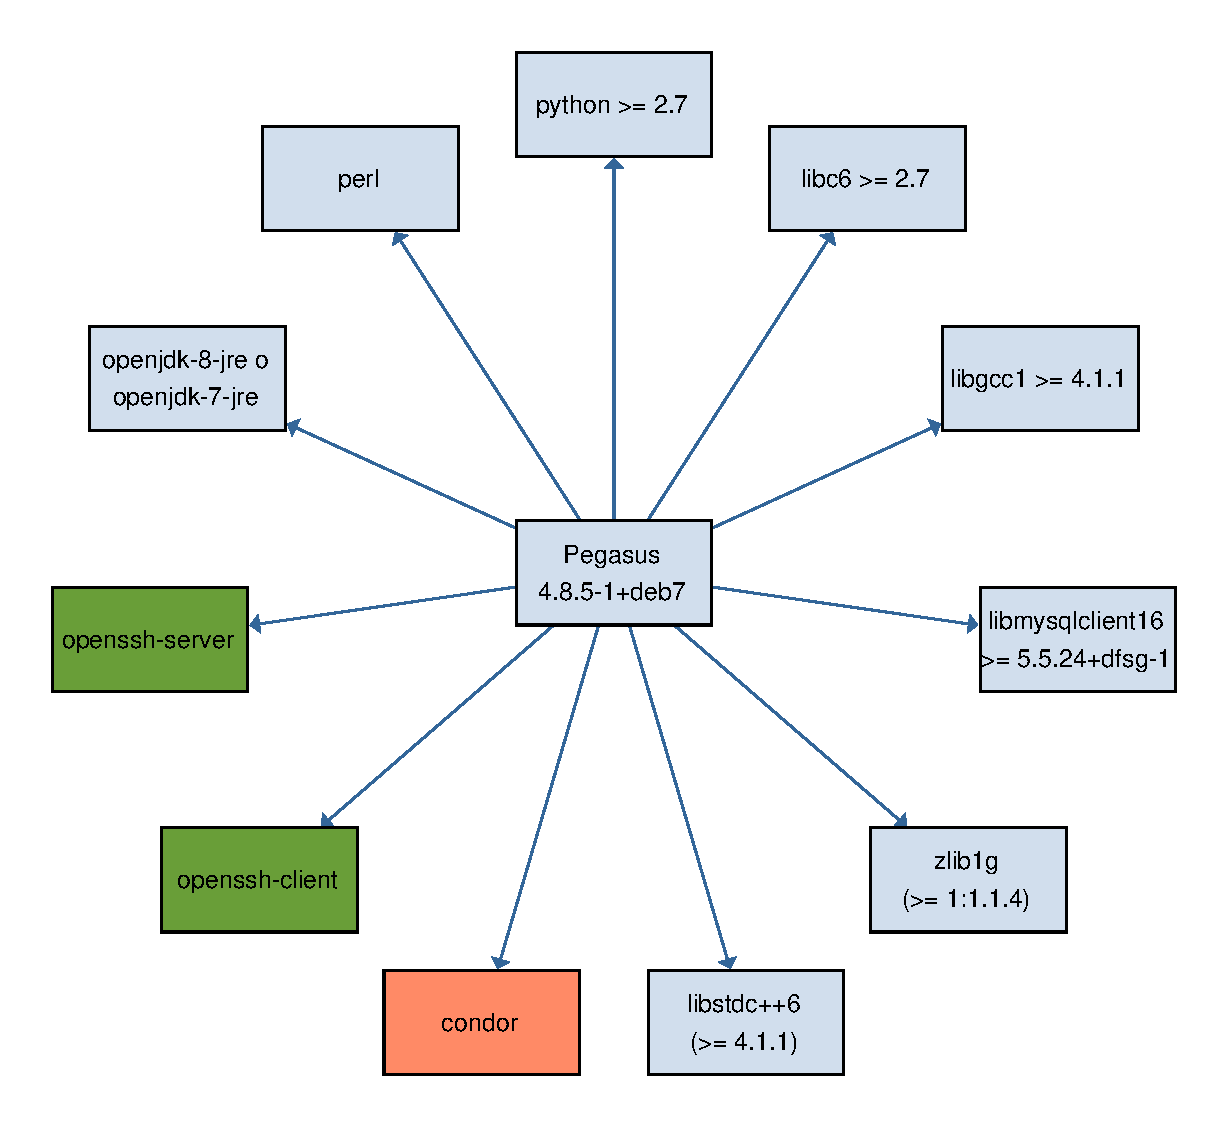
\includegraphics[width=.5\textwidth]{Figures/pegasus-deps}
\caption[Dependencias Pegasus]{Dependencias de Pegasus. En azul: dependencias necesarias y especificadas en el sistema de paquetes. En verde: necesarias pero no especificadas en el sistema de paquetes. En naranjas: dependencias recomendadas}
\label{fig:pegasus-deps}
\end{figure}

Las imágenes se encuentran disponibles en DockerHub~\footnote{\url{https://hub.docker.com/r/dockerpedia/pegasus_workflow_images/}}

\subsubsection{Soybean Knowledge Base}

El workflow SoyKB (Soybean Knowledge Base) \cite{joshi2012soybean} permite realizar un proceso de re-secuencia de germoplasma de la soya, con el objetivo de estudiar rasgos como aceites, proteína, resistencia de los nematodos del quiste de la soya y resistencia al estrés.
Pegasus entrega el workflow y implementa tres operaciones: polimorfismo de nucleótido único (SNP), la operación insertar/remover (indel) de la base del genoma del organismo y una análisis utilizando el software GATK \footnote{\url{https://software.broadinstitute.org/gatk/}}
La figura \ref{fig:soykb} muestra una representación gráfica del workflow, donde se realiza un análisis en paralelo de las muestras. Primero son alineadas con el genoma de referencia,  se identifica los indels y SNPs y luego se fusiona y filtra los resultados. 

\begin{figure}[t]
\centering
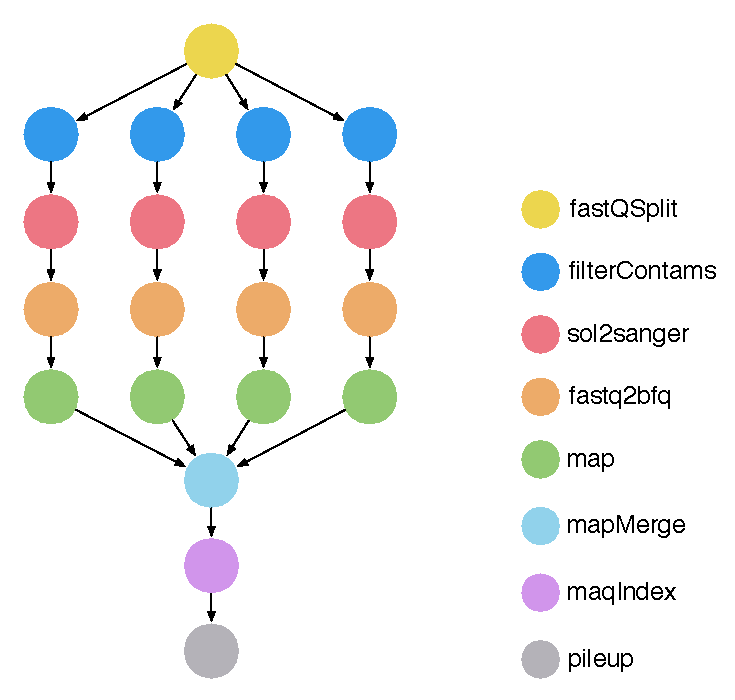
\includegraphics[width=.5\textwidth]{Figures/workflow-genome}
\caption[Representación workflow: SoyKb]{Representación entregada por Pegasus del workflow SoyKB.}\label{fig:soykb}
\end{figure}

Al estudiar la documentación de workflow SoyKB, se han obtenidos los siguientes componentes de software, que se clasifican en dos tipos: propio (en amarillo) y de terceros (en verde). Los componentes principales son: bwa, gatk y picard y el software de tercero java-1.7.0

\begin{figure}[t]
\centering
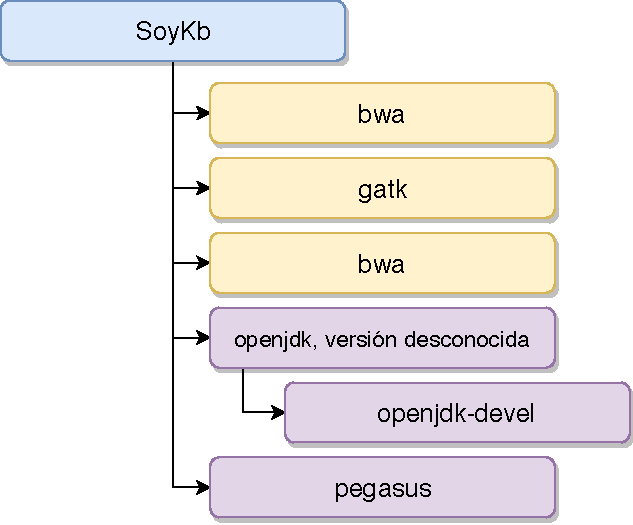
\includegraphics[width=.8\textwidth]{Figures/soykb-deps}
\caption[Dependencias workflow SoyKb]{Dependencias de SoyKb. En amarillo: software propio y en verde software de terceros}\label{fig:soykb-deps} 
\end{figure}

La evaluación de los resultados se realizó de forma manual al igual que en \cite{santana2017reproducibility} debido a los pasos aleatorios del workflow. La metodología de la verificación fue la revisión de la estructura de los resultados, el tamaño de los archivos, número de líneas y la inexistencia de errores.

\subsubsection{Montage}

Montage es un conjunto de herramientas creadas por \textit{NASA Infrared Processing and Analysis Center (IPAC)}, permitiendo generar bajo demanda mosaicos de imágenes astronómicas personalizadas, se utilizan archivos de entrada que cumplen con el estándar del Sistema de Transporte Flexible de Imágenes (FITS) y que contienen datos de imágenes registrados en proyecciones que cumplen con los estándares del Sistema Mundial de Coordenadas (WCS).

La figura \ref{fig:montage} entregada por Pegasus ilustra el workflow Montage. Cada uno de los nodos de la figura es un software binario que generan la imagen final.

Debido a que el software es un binario, no se encuentra empaquetado. Por lo tanto fue descargado de la fuente. Las direcciones de descargas se encuentran en el archivo de DockerFile \footnote{\url{https://github.com/dockerpedia/montage/blob/master/Dockerfile}}.  

\begin{figure}[t]
\centering
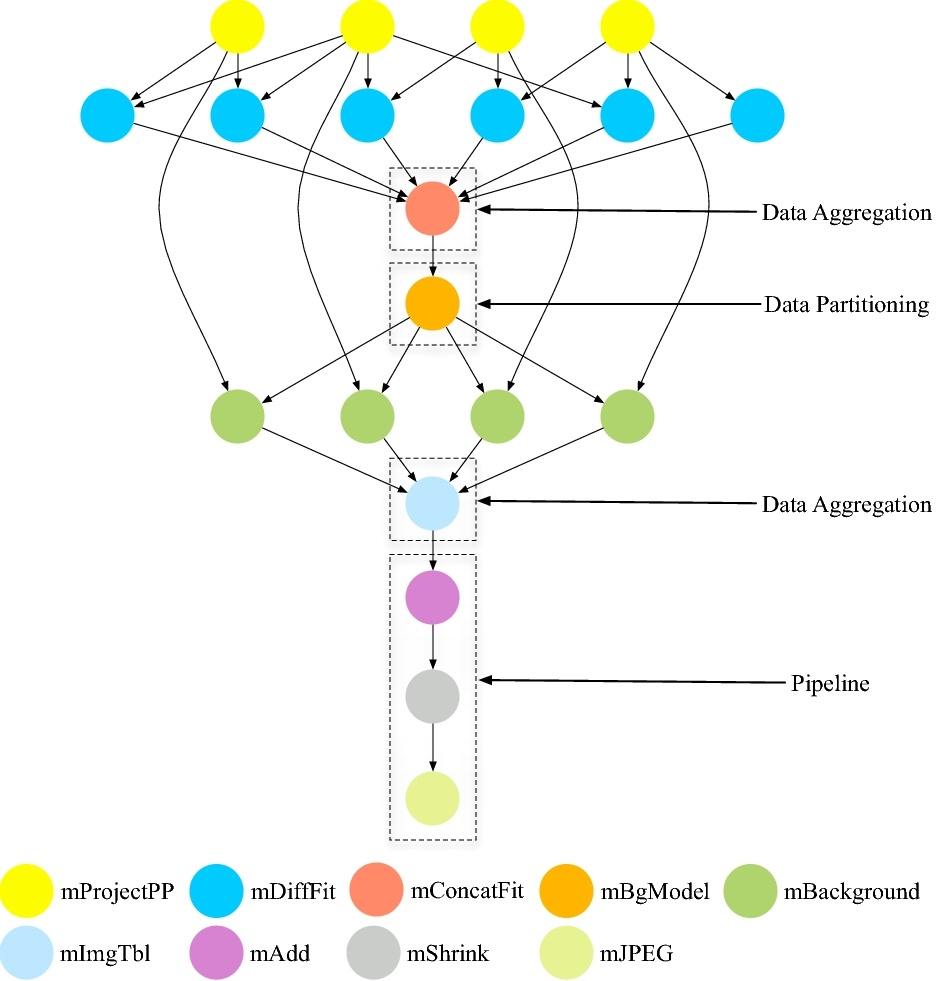
\includegraphics[width=.5\textwidth]{Figures/montage}
\caption[Representación workflow: Montage]{Representación entregada por Pegasus del workflow Montage. Cada uno de los nodos es una operación y la leyenda indica el nombre de la operación.}\label{fig:montage}
\end{figure}

Dado que los resultados de Montage son imágenes se utiliza la herramienta de hash perceptual \footnote{\url{http://phash.org}} para realizar la comparación entre la imagen reproducida (imagen del cielo de 0,1 grados) frente a la original.
Como resultado, se obtiene un factor de similitud de 1,0 (de 1,0) con un umbral de 0,85.
Las figuras \ref{fig:montage-wicus} y \ref{fig:montage-mosorio} muestran las imágenes resultantes y los archivos resultantes en formato FITS se encuentran en el repositorio de DockerPedia \footnote{\url{https://github.com/dockerpedia/montage_results}}. 

\begin{figure*}[t]
    \centering
    \begin{subfigure}[b]{0.4\textwidth}
         \centering
         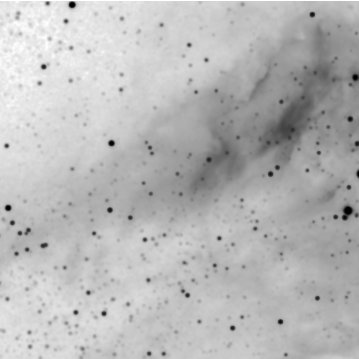
\includegraphics[width=\textwidth]{Figures/montage-original}
         \caption[Resultados workflow original: Montage]{Resultados originales obtenidos desde WICUS}
         \label{fig:montage-wicus}
     \end{subfigure}
         ~ 
	    \begin{subfigure}[b]{0.4\textwidth}
         \centering
         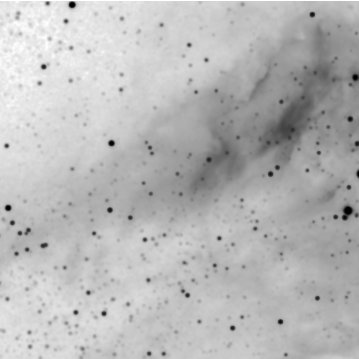
\includegraphics[width=\textwidth]{Figures/montage-mosorio}
         \caption[Resultados workflow reproducidos: Montage]{Resultados reproducidos por nuestra propuesta}
         \label{fig:montage-mosorio}
     \end{subfigure}
        \caption[Comparación resultados Montage]{Los resultados obtenidos con el nuevo ambiente son iguales}
        \label{fig:montage-results}
\end{figure*}



\subsection{dispel4py}

dispel4py ~\cite{DBLP:conf/eScience/FilgueiraKAKSS15} es una biblioteca Python para describir workflow para aplicaciones intensivas de datos, que luego se traducen y ejecutan en plataformas distribuidas (por ejemplo, Apache Storm, clusters MPI, etc.).
El paquete dispel4py ha sido obtenido del repositorio oficial \footnote{\url{https://github.com/rosafilgueira/dispel4py_workflows}}. 
Para la instalación el paquete, se utiliza Conda, un gestor de paquetes, dependencias y entornos para lenguajes Python, R, Ruby, Lua, Scala, Java, JavaScript, C/ C++, FORTRAN y que es ampliamente utilizado en entornos de \textit{Jupyter notebook}. 
Los principales requisitos de dispel4py obtenidos de la documentación son: Python2.7, git y  Python-setuptools
Las imágenes se encuentran disponibles en DockerHub~\footnote{\url{https://hub.docker.com/r/dockerpedia//}}



\subsubsection{Internal extinction}

\textit{Internal Extinction of Galaxies} workflow calcula la extinción interna de galaxias desde el catalogo Amiga. Estos datos son obtenidos a partir de un servicio llamado Observatorio Virtual, que es una red de herramientas y servicios que implementan estándares publicados por la \textit{International Virtual Observatory Alliance} (IVOA). El workflow calcula una propiedad, que representa la extinción de polvo dentro de las galaxias y que es un coeficiente de corrección necesario para calcular la luminosidad óptica de una galaxia.

El workflow primero lee el archivo de inicio que contiene la declinación y ascensión recta de 1051 galaxias. Luego, utiliza estos valores para realizar consultas al observatorio virtual. Los valores resultantes de las consultas son filtrados y se seleccionan sólo los valores que correspondan al tipo morfológico (Mtype) y al rango de los ejes del isófito 25 $mag/arcsec^{2}$ (logr25) de las galaxias. Finalmente, se calcula su extinción interna. La figura \ref{fig:internal} muestra los pasos del workflow

\begin{figure}[t]
\centering
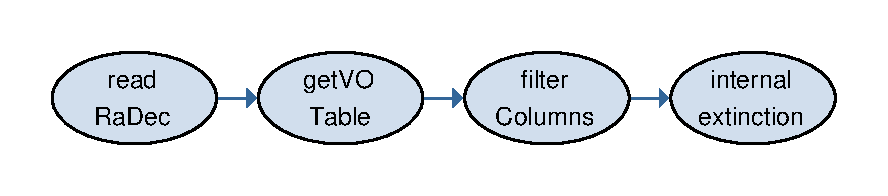
\includegraphics[width=.8\textwidth]{Figures/internal-extinction}
\caption[Representación workflow: Internal Extinction]{Pasos necesarios para el workflow Internal Extinction}\label{fig:internal}
\end{figure}

Nuestra investigación inicial sobre las dependencias para la ejecución de Internal extinction muestra que el software principal requeridos es el siguiente:  \verb|requests|, \verb|python=|, \verb|numpy| y \verb|astropy|

\subsubsection{Seismic Ambient Noise Cross-Correlation}
\textit{Seismic Ambient Noise Cross-Correlation workflow} (o xcorr workflow) es parte del proyecto \textit{Virtual Earthquake and seismology Research Community e-science environment in Europe} (VERCE). 
El objetivo del workflow es la previsión de riesgos producidos por terremotos y erupciones volcánicas. Estos eventos en ciertos casos van precedidos o acompañados de cambios en las propiedades geofísicas de la Tierra, como la velocidad de las olas o la velocidad de los eventos. 

Para lograr desarrollo de métodos fiables de evaluación de riesgos para estas amenazas se requiere un análisis en tiempo real de los datos sísmicos y un pronóstico verdaderamente prospectivo y pruebas para reducir los sesgos.

\texttt{xcorr} logra lo anterior a través de dos etapas, la primera etapa es un pre-procesamiento de series de tiempo de una estación sísmica llamadas trazas, en esta etapa se realiza una serie de tratamientos y el procesamiento de cada traza es independiente del procesamiento de otras trazas, haciendo que esta fase sea paralela. 
Luego la segunda etapa empareja todas las estaciones y calcula la correlación cruzada para cada par. La figura \ref{fig:xcorr} muestra los pasos del workflow.


\begin{figure}[t]
\centering
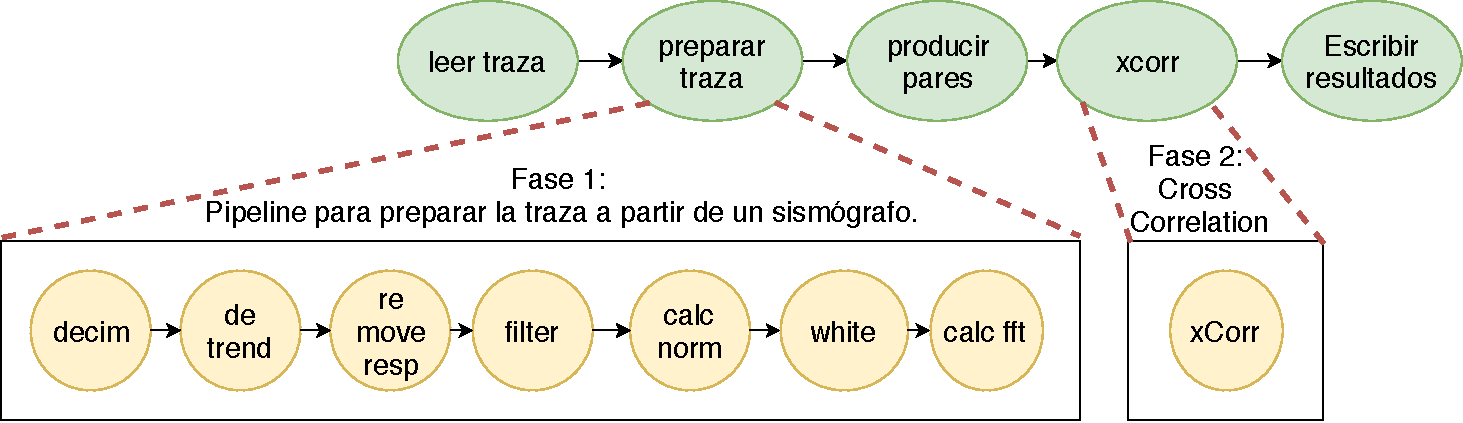
\includegraphics[width=.8\textwidth]{Figures/xcorr}
\caption[Representación workflow: Seismic Ambient Noise Cross-Correlation]{Representación workflow: Seismic Ambient Noise Cross-Correlation}\label{fig:xcorr}
\end{figure}


Nuestra investigación inicial sobre las dependencias para la ejecución indica que los componentes de software necesarios son: \verb|python|, \verb|obspy| y \verb|numpy|


\subsection{WINGS}

WINGS es un sistema de flujo de trabajo semántico que ayuda a los científicos en el diseño de experimentos computacionales. 
En WINGS, se especifica cómo deben ser procesados los conjuntos de datos por una serie de componentes del software en una configuración particular.
WINGS a diferencia de los otros sistemas de workflows utiliza imágenes Docker para su distribución. Pese a que WINGS presenta las imágenes de Docker, estas imágenes son una caja negra y no es posible obtener los componentes de software.
La investigación inicial sobre las dependencias indica que los principales requisitos de WINGS son: Java 1.8, Tomcat 8.5, Docker. La figura \ref{fig:wings-deps} muestra en mayor detalles las dependencias especificadas tanto por el sistema de paquetes o documentación.

\begin{figure}[t]
\centering
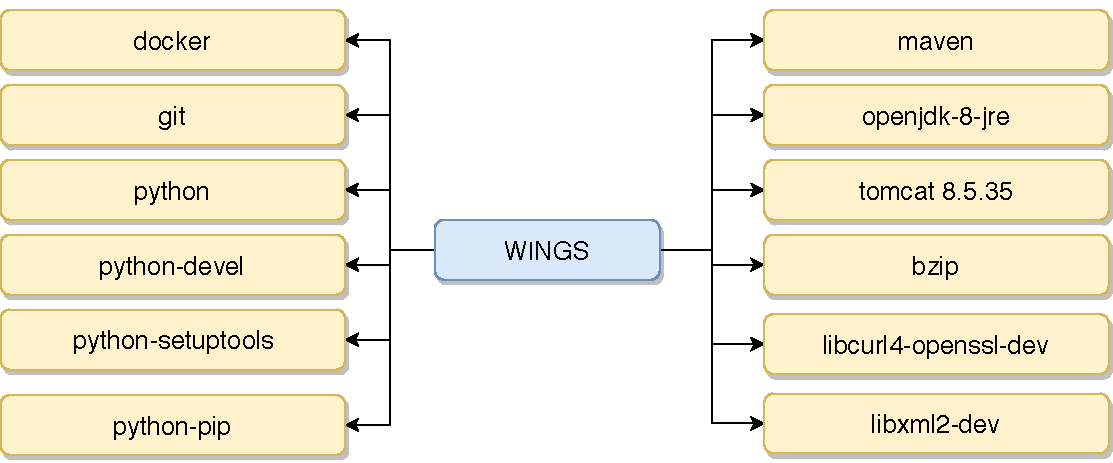
\includegraphics[width=.8\textwidth]{Figures/wings-deps}
\caption{Dependencias de WINGS}\label{fig:wings-deps}
\end{figure}

Las imágenes se encuentran disponibles en DockerHub~\footnote{\url{https://hub.docker.com/r/dockerpedia/wings/}}


\subsubsection{MODFLOW-NWT}

MODFLOW es el modelo hidrológico modular del \textit{United States Geological Survey}~\footnote{\url{https://www.usgs.gov}} (USGS). MODFLOW se considera una norma internacional para simular y predecir las condiciones de las aguas subterráneas y las interacciones entre las aguas subterráneas y superficiales.
El USGS MODFLOW-NWT es una formulación de Newton-Raphson para MODFLOW-2005 con el objetivo de mejorar la solución de problemas de flujo, secado y humectación de aguas subterráneas no confinadas.

\begin{figure}[t]
\centering
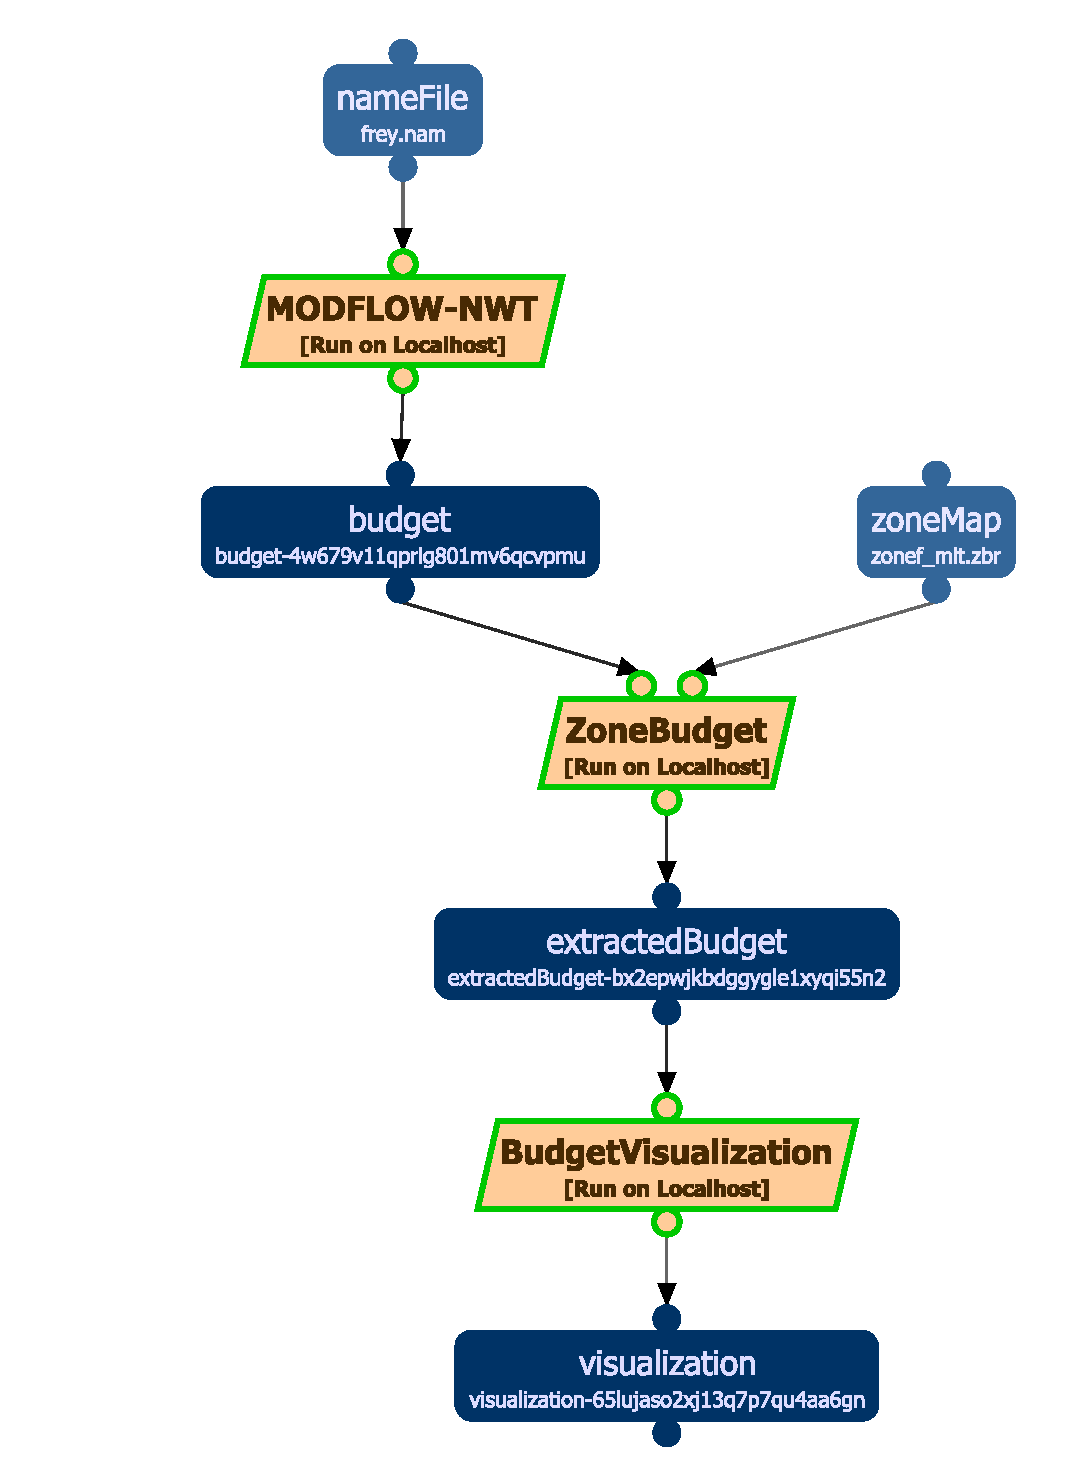
\includegraphics[width=0.6\textwidth]{Figures/usgs-modflow-nwt}
\caption{Representación workflow: MODFLOW-NWT}
\label{fig:modflow}
\end{figure}


La figura \ref{fig:modflow} muestra la estructura principal del workflow, desarrollado con pipeline compuesto por tres pasos. El proceso inicia leyendo el modelo a utilizar. Luego, el archivo de zona se usa para especificar arreglos de zonas que van usarse y finalmente se genera una visualización que muestra la cantidad de millones de galones por día en zona. Las figuras \ref{fig:modflow-original} y \ref{fig:modflow-reproduced} muestran los resultados generados por el ambiente original y reproducido respectivamente.

\begin{figure*}[t]
    \centering
    \begin{subfigure}[b]{\textwidth}
         \centering
         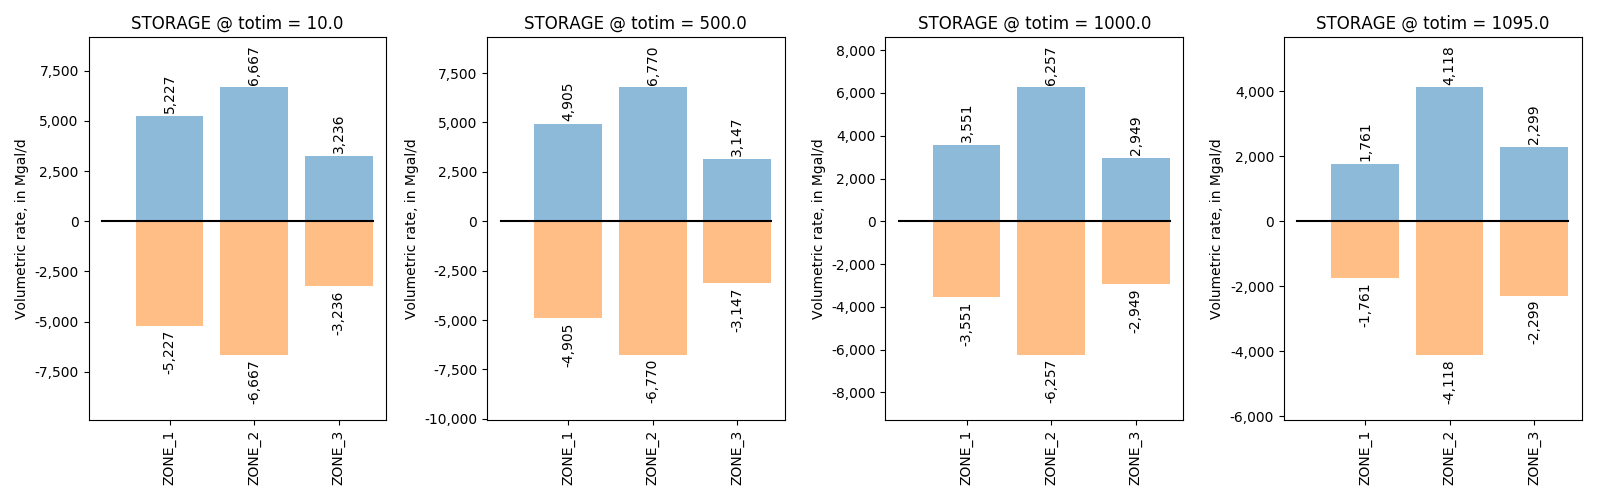
\includegraphics[width=\textwidth]{Figures/viz-original}
         \caption[Resultados workflow originales: ModFlow]{Resultados originales entregados por el Information Sciences Institute}
         \label{fig:modflow-original}
     \end{subfigure}
	
	    \begin{subfigure}[b]{\textwidth}
         \centering
         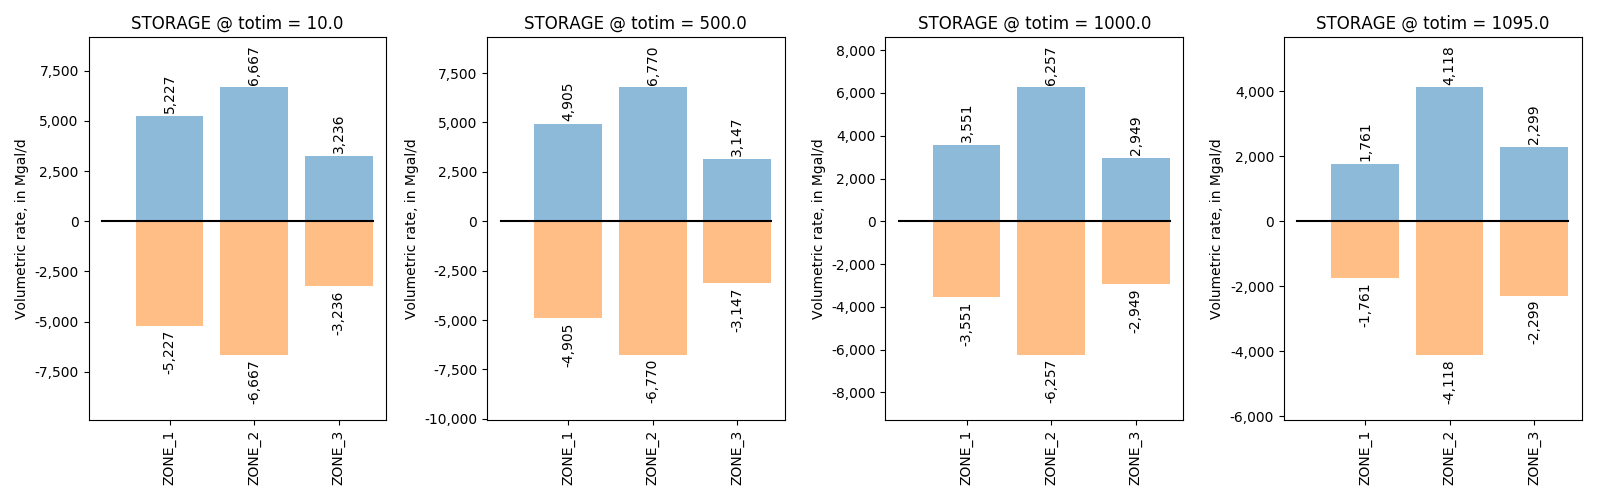
\includegraphics[width=\textwidth]{Figures/viz-reproduced}
        \caption[Resultados workflow reproducidos: ModFlow]{Resultados reproducidos por nuestra propuesta}
         \label{fig:modflow-reproduced}
     \end{subfigure}
        \caption[Comparación resultados MODFLOW-NEW]{Los resultados obtenidos son idénticos}
        \label{fig:both-modflow}
\end{figure*}






%-----------------------------------------------
% 5.2 Physical conservation
%-----------------------------------------------
\section{Conservación física}\label{s5.2}

Todas las imágenes son publicadas con su correspondiente Dockerfile y cualquier usuario puede inspeccionarlas y mejorarlas. Las imágenes puede ser encontradas en DockerHub \footnote{https://hub.docker.com/u/dockerpedia/} y GitHub \footnote{\url{https://github.com/dockerpedia}}. 

Para evaluar la conservación física se utiliza tres proveedores diferentes: DigitalOcean, Google Cloud y un local. La figura de \ref{image-env} presenta una descripción de las características de los ambientes    

\begin{table}[t]
\centering
\begin{tabular}{|l|l|l|l|}
\hline
Resource   & Digital Ocean & Google Compute & Local     \\ \hline
RAM (GB)   & 8             & 8              & 4         \\ \hline
Disk (GB)  & 100           & 100            & 70        \\ \hline
CPU (GHz)  & 2.0           & 2.5            & 2.8          \\ \hline
CPU (Cores)& 4             & 2              & 4          \\ \hline
CPU (Arch) & 64            & 64             & 64        \\ \hline
OS         & Centos 7      & Debian 9       & Fedora 27 \\ \hline
\end{tabular}
\caption{Características de hardware de pruebas.}
\label{image-env}
\end{table}

El ambiente debe tener instalado Docker, cada imagen en su manifiesto describe la versión de Docker con cuál fue construida. Sin embargo, Docker asegura idempontencia para los ambientes CentOS7, Debian 10/9/8/7.7, Fedora 26/27/28, Ubuntu 14.04/16.06/18.04, Windows 10, macOS El Capitan 10.11 o nuevas versiones.
El proceso de instalación puede ser encontrado en la documentación oficial \footnote{\url{https://docs.docker.com/install/}}.

Cada imagen de Docker tiene archivo README con las instrucciones para correr el experimento. Las figuras \ref{lst:1}~\ref{lst:2} y~\ref{lst:3}  muestran los pasos necesarios para correr el experimento computacional: SoyKB. 

El primer paso es correr el experimento y descargar la imagen:
\begin{figure*}[ht]
\begin{lstlisting}[caption={Descargar y correr la imagen disponible en DockerHub mosorio/pegasus\_workflow\_images:soykb},label={lst:1},language=bash]
docker run -d --rm -it --name soybean \
 mosorio/pegasus_workflow_images:soykb
\end{lstlisting}	
\end{figure*}


Luego, el usuario debe entrar al container. El usuario puede confirmar que se encuentra dentro del container por el cambio de símbolo de la terminal  (prompt).
\begin{figure*}[ht]
\begin{lstlisting}[caption={Entrar al ambiente computacional utilizando bash},label={lst:2},language=bash]
root@docker-instance:~# docker exec \
-ti -u workflow:workflow soybean bash
workflow@a0f861e6fbc4:~ 
\end{lstlisting}
\end{figure*}

Finalmente, correr el workflow. 

\begin{figure*}[ht]
\begin{lstlisting}[caption={Run the workflow},label={lst:3},language=bash]
workflow@a0f861e6fbc4:~/soykb \
./workflow-generator --exec-env distributed	
\end{lstlisting}
\end{figure*}

Para evaluar si las imágenes Docker son livianas y almacenables, se construyeron dos imágenes, una utilizando Docker y otra utilizando máquinas virtuales. La imagen de Docker se construyó bajo nuestro enfoque y la imagen de la máquina virtual basada en el trabajo de ~\cite{santana2017reproducibility}. Luego se compara el uso de disco de ambas.

%-------------------------------------------
% Logical conservation
%-----------------------------------------------
\section{Conservación lógica}\label{s5.3}

A través de las anotaciones realizadas, se busca describir los ambientes computacionales en forma automática, comparar las diferencias entre dos ambientes y construir un ambiente computacional similar que permita reproducir la ejecución del workflow. 

Para ello, se anota de automática los workflows con nuestra herramienta, las anotaciones están agrupadas por: pasos de construcción y componentes de software. 

Para evaluar la calidad de las anotaciones se utilizan dos experimentos.

\begin{itemize}
	\item Reproducir el ambiente utilizando los pasos de construcción representados por DeploymentPlan.
	\item Detectar las similitudes y diferencias entre dos ambientes computacionales.
\end{itemize}

Para obtener las anotaciones, se propone e implementa usar Clair y construir un sistema de anotador. La figura \ref{fig:arch} muestra los pasos principales del sistema.

\begin{figure*}[t]
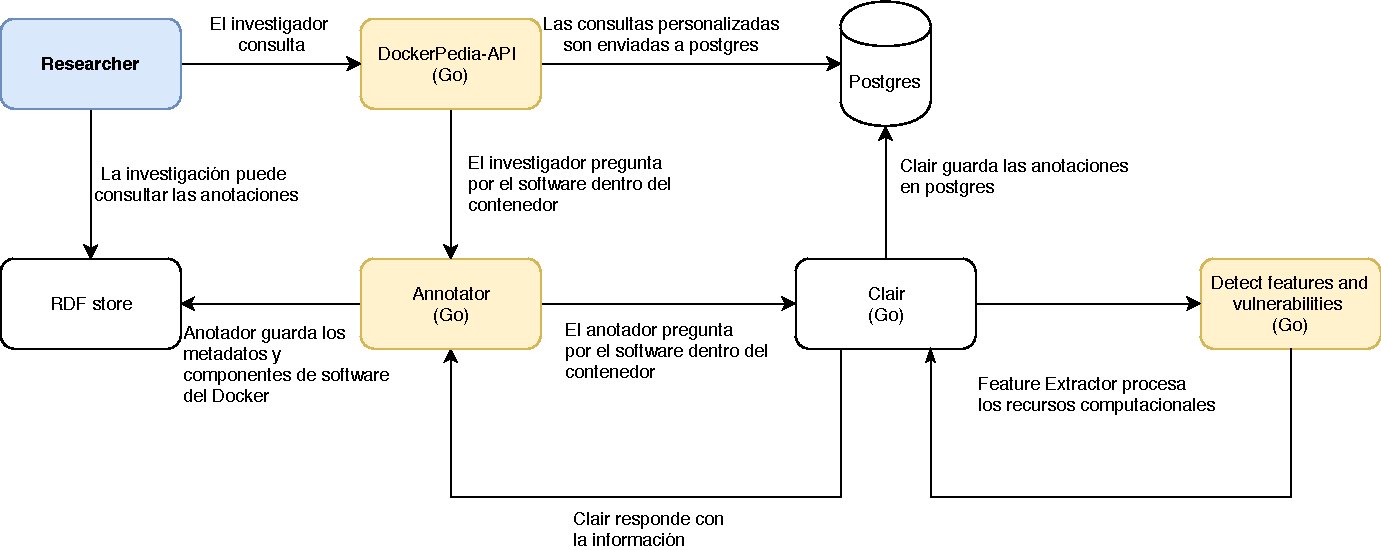
\includegraphics[width=\textwidth]{Figures/arch.pdf}
\caption[Arquitectura sistema anotador]{El sistema anotador permite recibir la información de la imagen, consultar los componentes de software a nuestra versión de Clair, obtener metadatos desde el manifesto y almacenar la información en forma de triples en Apache Jena.}\label{fig:arch}
\end{figure*}


\begin{enumerate}
    \item El investigador pregunta sobre la información de una imagen al sistema anotador. El sistema anotador se encuentra escrito en GoLang y disponible en nuestro repositorio.
    \item El sistema anotador pregunta a Clair sobre software y sus vulnerabilidades de la imagen. El sistema de Clair es una versión propia que puede detectar componentes de software instalado por Conda.
    \item Para obtener los pasos de construcción, etiquetas, arquitectura y más información. El anotador obtiene el manifiesto de la imagen desde DockerHub
    \item El sistema anotador guarda la información usando RDF y la ontología propuesta.
\end{enumerate}


Para reproducir el entorno, el sistema obtiene el repositorio asociado a la imagen y construye la nueva imagen. La URL del repositorio y el cambio asociado (representado por un VCS commit) se pueden obtener por dos métodos: consultando nuestras anotaciones o usando un comando Docker. El listado \ref{lst:inspect_command} muestra las etiquetas de la imagen de flujo de trabajo SoyKB.

\begin{figure*}
\begin{lstlisting}[caption={Inspect image annotations},label={lst:inspect_command},language=bash]
root@docker-instance:~# docker inspect \ 
    --format='{{json .Config.Labels}}' \ 
    dockerpedia/soykb:latest
\end{lstlisting}
\end{figure*}

La figura \ref{lst:inspect_result} muestra algunas de las etiquetas de la imagen basado en \textit{Open Container Initiative}. Y todas las imágenes disponibles en nuestros repositorios presentan esas etiquetas.

\begin{figure*}
\begin{lstlisting}[caption={Inspect image annotations},label={lst:inspect_result},language=json]
{
"maintainer": "Maximiliano Osorio <mosorio@inf.utfsm.cl>",
"org.label-schema.build-date": "2018-11-10T21:11:28Z",
"org.label-schema.name": "Soybean Knowledge Base",
"org.label-schema.schema-version": "1.0",
"org.label-schema.url": "http://www.soykb.org/",
"org.label-schema.vcs-ref": "15955b0",
"org.label-schema.vcs-url": "https://github.com/dockerpedia/soykb",
"org.label-schema.vendor": "DockerPedia",
"org.label-schema.version": "1.0"
}

\end{lstlisting}
\end{figure*}


Para evaluar si los entornos son similares, comparamos ambas imágenes utilizando el lenguaje de consulta SPARQL 1.1. El experimento fue un caso real en el que una imagen podía ejecutar el flujo de trabajo y la otra no. 
La figura \ref{lst:compare_query} muestra la consulta para identificar los componentes diferentes de software entre dos imágenes y la figura \ref{lst:compare_query_2} muestra muestra la consulta para identificar los componentes iguales de software entre dos imágenes.
\begin{figure*}
\begin{lstlisting}[caption={¿Cuáles son los diferentes componentes entre dos imágenes?},label={lst:compare_query},language=sparql]
SELECT * WHERE {
 pegasus_workflow_images%3Alatest
  vocab:containsSoftware ?p .
 MINUS{
 pegasus_workflow_images%3Apegasus-4.8.5
  vocab:containsSoftware ?p   
 }
}
\end{lstlisting}
\end{figure*}

\begin{figure*}

\begin{lstlisting}[caption={¿Cuáles son los componentes que comparten entre dos imágenes?},label={lst:compare_query_2},language=sparql]
SELECT * WHERE {
 pegasus_workflow_images%3Alatest
      vocab:containsSoftware ?p .
 pegasus_workflow_images%3Apegasus-4.8.5
      vocab:containsSoftware ?p   
    }
    \end{lstlisting}
    \end{figure*}

    
\section{Resultados y discusión}\label{s5.4}
Se logró ejecutar los workflows utilizando imágenes Docker sobre sus plataformas correspondientes.
Todas las ejecuciones se compararon con la imagen VM predefinida, donde ya existía un entorno de ejecución. Los resultados muestran que los ambientes de ejecución de contenedores son capaces de ejecutar completamente sus workflow relacionados. Se  comprobó que no sólo los workflows se ejecutan con éxito, sino también que los resultados son correctos y equivalentes a través de los datos de salida producidos. 

Por otra parte, los resultados experimentales muestran que nuestra propuesta puede detectar automáticamente los componentes del software, las vulnerabilidades relacionadas, los pasos de construcción y los metadatos específicos de los experimentos científicos en forma de imágenes Docker. 
Además, los resultados muestran que es posible extender Clair para anotar a otros gestores de paquetes. 

Las anotaciones generadas por nuestro enfoque permiten comparar los componentes de software entre dos o más entornos. Esta función se puede utilizar como herramienta de depuración cuando un entorno reproducido no funciona.
Por ejemplo, en agosto de 2018, se construyó la imagen del workflow SoyKB, y se pudo ejecutar el workflow con éxito. Sin embargo, se reconstruyó una nueva imagen en noviembre con el mismo DeploymentPlan y no se pudo ejecutar el workflow con éxito.


Se utilizaron las anotaciones de los componentes de software dentro de ambas imágenes. Y se encontró las siguientes diferencias:
\begin{itemize}
    \item Agosto: Pegasus 4.8 y Java 1.7
    \item Noviembre: Pegasus 4.9 y Java 1.8
\end{itemize}

Luego se analizó el código y la documentación de SoyKB y las dependencias de Pegasus 4.9. Como resultado, se obtuvo las gráficas de dependencia mostradas en la figura \ref{fig:pegasus49}.  Los gráficos de dependencia muestran que el paquete Pegasus 4.9 y SoyKB no son compatibles debido a sus requerimientos de versión Java.

Y construyó una nueva imagen instalando Pegasus 4.8, y se obtuvo los gráficos de dependencia que se muestran en la figura \ref{fig:pegasus48}. Aquí, el gráfico no tiene un conflicto y se pudo ejecutar el workflow con éxito.

La nueva imagen fue nombrada como: \verb|pegasus_workflow_images:4.8.5|


\begin{figure*}[t]
    \centering
    \begin{subfigure}[b]{0.40\textwidth}
         \centering
         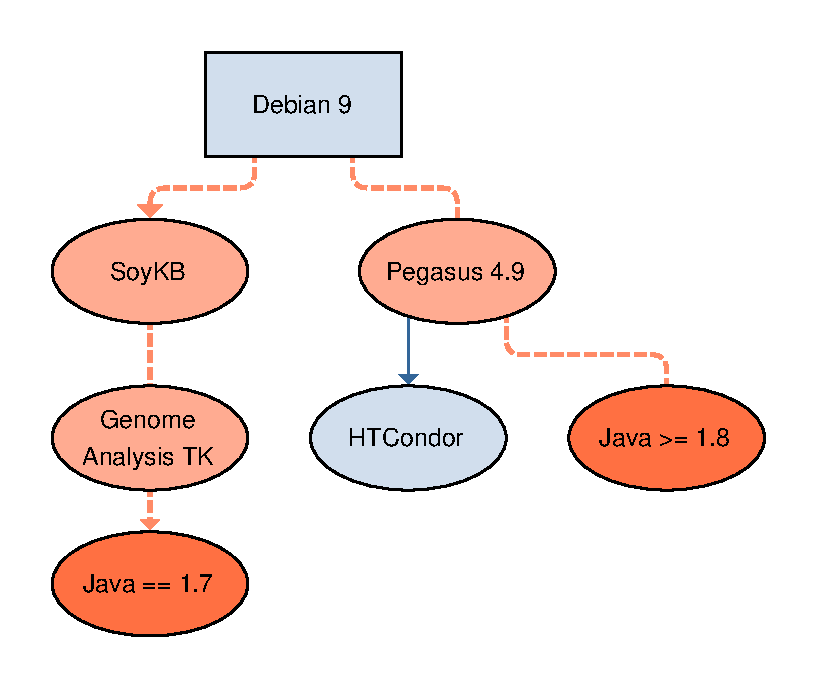
\includegraphics[width=\textwidth]{Figures/pegasus-49.pdf}
         \caption{Gráfico de dependencias Pegasus 4.9 y SoyKB}
         \label{fig:pegasus49}
     \end{subfigure}
    ~ 
    \begin{subfigure}[b]{0.40\textwidth}
         \centering
         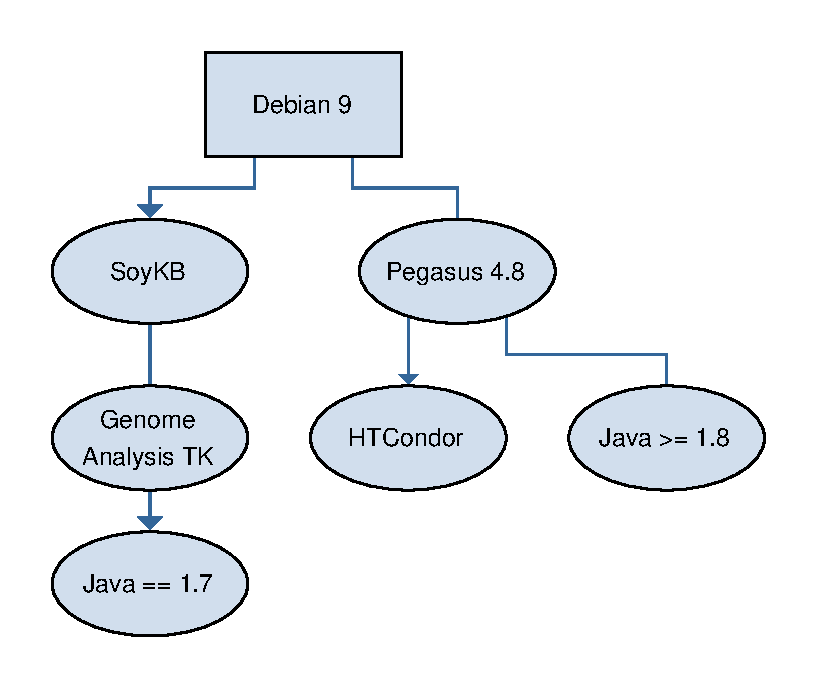
\includegraphics[width=\textwidth]{Figures/pegasus-48.pdf}
         \caption{Gráfico de dependencias Pegasus 4.8 y SoyKB}
         \label{fig:pegasus48}
     \end{subfigure}
        \caption{Análisis de dependencias imágenes Pegasus}
        \label{fig:dependencies-graph}
\end{figure*}

La razón principal de los trabajos anteriores para evitar la conservación física era la gran demanda de almacenamiento de máquinas virtuales. 
Los resultados de la comparación del uso del disco muestran que hay una disminución del 64,2\% para la imagen Pegasus y del 41,5\% para la dispel4py. La tabla \ref{storage-reduce} muestra la diferencia para el sistema de flujo de trabajo Pegasus y dispel4py.


\begin{table}[t]
\centering
\begin{tabular}{|l|l|l|}
\hline
Enfoque        & Pegasus (MB) & dispel4py (MB) \\ \hline
Virtualization & 1929         & 3509 \\ \hline
Container      & 690          & 2500 \\ \hline
\end{tabular}
\caption[Comparación de uso de disco entre VMs y contenedores]{Uso de disco de las imágenes pegasus y dispel4py utilizando máquinas virtuales y contenedores}
\label{storage-reduce}
\end{table}
